%\documentclass[12pt]{article}
\documentclass[12pt,landscape]{article}


%packages
%\usepackage{latexsym}
\usepackage{graphicx}
\usepackage{color}
\usepackage{amsmath}
\usepackage{dsfont}
\usepackage{placeins}
\usepackage{amssymb}
\usepackage{wasysym}
\usepackage{abstract}
\usepackage{hyperref}
\usepackage{etoolbox}
\usepackage{datetime}
\usepackage{xcolor}
\usepackage{alphalph}
\settimeformat{ampmtime}

%\usepackage{pstricks,pst-node,pst-tree}

%\usepackage{algpseudocode}
%\usepackage{amsthm}
%\usepackage{hyperref}
%\usepackage{mathrsfs}
%\usepackage{amsfonts}
%\usepackage{bbding}
%\usepackage{listings}
%\usepackage{appendix}
\usepackage[margin=1in]{geometry}
%\geometry{papersize={8.5in,11in},total={6.5in,9in}}
%\usepackage{cancel}
%\usepackage{algorithmic, algorithm}

\makeatletter
\def\maxwidth{ %
  \ifdim\Gin@nat@width>\linewidth
    \linewidth
  \else
    \Gin@nat@width
  \fi
}
\makeatother

\definecolor{fgcolor}{rgb}{0.345, 0.345, 0.345}
\newcommand{\hlnum}[1]{\textcolor[rgb]{0.686,0.059,0.569}{#1}}%
\newcommand{\hlstr}[1]{\textcolor[rgb]{0.192,0.494,0.8}{#1}}%
\newcommand{\hlcom}[1]{\textcolor[rgb]{0.678,0.584,0.686}{\textit{#1}}}%
\newcommand{\hlopt}[1]{\textcolor[rgb]{0,0,0}{#1}}%
\newcommand{\hlstd}[1]{\textcolor[rgb]{0.345,0.345,0.345}{#1}}%
\newcommand{\hlkwa}[1]{\textcolor[rgb]{0.161,0.373,0.58}{\textbf{#1}}}%
\newcommand{\hlkwb}[1]{\textcolor[rgb]{0.69,0.353,0.396}{#1}}%
\newcommand{\hlkwc}[1]{\textcolor[rgb]{0.333,0.667,0.333}{#1}}%
\newcommand{\hlkwd}[1]{\textcolor[rgb]{0.737,0.353,0.396}{\textbf{#1}}}%

\usepackage{framed}
\makeatletter
\newenvironment{kframe}{%
 \def\at@end@of@kframe{}%
 \ifinner\ifhmode%
  \def\at@end@of@kframe{\end{minipage}}%
  \begin{minipage}{\columnwidth}%
 \fi\fi%
 \def\FrameCommand##1{\hskip\@totalleftmargin \hskip-\fboxsep
 \colorbox{shadecolor}{##1}\hskip-\fboxsep
     % There is no \\@totalrightmargin, so:
     \hskip-\linewidth \hskip-\@totalleftmargin \hskip\columnwidth}%
 \MakeFramed {\advance\hsize-\width
   \@totalleftmargin\z@ \linewidth\hsize
   \@setminipage}}%
 {\par\unskip\endMakeFramed%
 \at@end@of@kframe}
\makeatother

\definecolor{shadecolor}{rgb}{.77, .77, .77}
\definecolor{messagecolor}{rgb}{0, 0, 0}
\definecolor{warningcolor}{rgb}{1, 0, 1}
\definecolor{errorcolor}{rgb}{1, 0, 0}
\newenvironment{knitrout}{}{} % an empty environment to be redefined in TeX

\usepackage{alltt}
\usepackage[T1]{fontenc}

\newcommand{\qu}[1]{``#1''}
\newcounter{probnum}
\setcounter{probnum}{1}

%create definition to allow local margin changes
\def\changemargin#1#2{\list{}{\rightmargin#2\leftmargin#1}\item[]}
\let\endchangemargin=\endlist 

%allow equations to span multiple pages
\allowdisplaybreaks

%define colors and color typesetting conveniences
\definecolor{gray}{rgb}{0.5,0.5,0.5}
\definecolor{black}{rgb}{0,0,0}
\definecolor{white}{rgb}{1,1,1}
\definecolor{blue}{rgb}{0.5,0.5,1}
\newcommand{\inblue}[1]{\color{blue}#1 \color{black}}
\definecolor{green}{rgb}{0.133,0.545,0.133}
\newcommand{\ingreen}[1]{\color{green}#1 \color{black}}
\definecolor{yellow}{rgb}{1,1,0}
\newcommand{\inyellow}[1]{\color{yellow}#1 \color{black}}
\definecolor{orange}{rgb}{0.9,0.649,0}
\newcommand{\inorange}[1]{\color{orange}#1 \color{black}}
\definecolor{red}{rgb}{1,0.133,0.133}
\newcommand{\inred}[1]{\color{red}#1 \color{black}}
\definecolor{purple}{rgb}{0.58,0,0.827}
\newcommand{\inpurple}[1]{\color{purple}#1 \color{black}}
\definecolor{backgcode}{rgb}{0.97,0.97,0.8}
\definecolor{Brown}{cmyk}{0,0.81,1,0.60}
\definecolor{OliveGreen}{cmyk}{0.64,0,0.95,0.40}
\definecolor{CadetBlue}{cmyk}{0.62,0.57,0.23,0}

%define new math operators
\DeclareMathOperator*{\argmax}{arg\,max~}
\DeclareMathOperator*{\argmin}{arg\,min~}
\DeclareMathOperator*{\argsup}{arg\,sup~}
\DeclareMathOperator*{\arginf}{arg\,inf~}
\DeclareMathOperator*{\convolution}{\text{\Huge{$\ast$}}}
\newcommand{\infconv}[2]{\convolution^\infty_{#1 = 1} #2}
%true functions

%%%% GENERAL SHORTCUTS

%shortcuts for pure typesetting conveniences
\newcommand{\bv}[1]{\boldsymbol{#1}}

%shortcuts for compound constants
\newcommand{\BetaDistrConst}{\dfrac{\Gamma(\alpha + \beta)}{\Gamma(\alpha)\Gamma(\beta)}}
\newcommand{\NormDistrConst}{\dfrac{1}{\sqrt{2\pi\sigma^2}}}

%shortcuts for conventional symbols
\newcommand{\tsq}{\tau^2}
\newcommand{\tsqh}{\hat{\tau}^2}
\newcommand{\sigsq}{\sigma^2}
\newcommand{\sigsqsq}{\parens{\sigma^2}^2}
\newcommand{\sigsqovern}{\dfrac{\sigsq}{n}}
\newcommand{\tausq}{\tau^2}
\newcommand{\tausqalpha}{\tau^2_\alpha}
\newcommand{\tausqbeta}{\tau^2_\beta}
\newcommand{\tausqsigma}{\tau^2_\sigma}
\newcommand{\betasq}{\beta^2}
\newcommand{\sigsqvec}{\bv{\sigma}^2}
\newcommand{\sigsqhat}{\hat{\sigma}^2}
\newcommand{\sigsqhatmlebayes}{\sigsqhat_{\text{Bayes, MLE}}}
\newcommand{\sigsqhatmle}[1]{\sigsqhat_{#1, \text{MLE}}}
\newcommand{\bSigma}{\bv{\Sigma}}
\newcommand{\bSigmainv}{\bSigma^{-1}}
\newcommand{\thetavec}{\bv{\theta}}
\newcommand{\thetahat}{\hat{\theta}}
\usepackage{accents}
\newlength{\dhatheight}
\newcommand{\doublehat}[1]{%
    \settoheight{\dhatheight}{\ensuremath{\hat{#1}}}%
    \addtolength{\dhatheight}{-0.35ex}%
    \hat{\vphantom{\rule{1pt}{\dhatheight}}%
    \smash{\hat{#1}}}}

\newcommand{\thetahathat}{\doublehat{\theta}}
\newcommand{\thetahatmm}{\hat{\theta}^{\mathrm{MM}}}
\newcommand{\thetahathatmm}{\thetahathat^{\mathrm{MM}}}
\newcommand{\thetahatmle}{\hat{\theta}^{\mathrm{MLE}}}
\newcommand{\thetahathatmle}{\thetahathat^{\mathrm{MLE}}}
\newcommand{\thetavechatmle}{\hat{\thetavec}^{\mathrm{MLE}}}
\newcommand{\muhat}{\hat{\mu}}
\newcommand{\musq}{\mu^2}
\newcommand{\muvec}{\bv{\mu}}
\newcommand{\muhatmle}{\muhat_{\text{MLE}}}
\newcommand{\lambdahat}{\hat{\lambda}}
\newcommand{\lambdahatmle}{\lambdahat_{\text{MLE}}}
\newcommand{\etavec}{\bv{\eta}}
\newcommand{\alphavec}{\bv{\alpha}}
\newcommand{\minimaxdec}{\delta^*_{\mathrm{mm}}}
\newcommand{\ybar}{\bar{y}}
\newcommand{\ybarT}{\bar{y}_T}
\newcommand{\ybarC}{\bar{y}_C}
\newcommand{\YbarT}{\bar{Y}_T}
\newcommand{\YbarC}{\bar{Y}_C}
\newcommand{\xbar}{\bar{x}}
\newcommand{\Xbar}{\bar{X}}
\newcommand{\phat}{\hat{p}}
\newcommand{\Phat}{\hat{P}}
\newcommand{\Zbar}{\bar{Z}}
\newcommand{\iid}{~{\buildrel iid \over \sim}~}
\newcommand{\inddist}{~{\buildrel ind \over \sim}~}
\newcommand{\approxdist}{~{\buildrel \cdot \over \sim}~}
\newcommand{\equalsindist}{~{\buildrel d \over =}~}
\newcommand{\loglik}[1]{\ell\parens{#1}}
\newcommand{\thetahatkminone}{\thetahat^{(k-1)}}
\newcommand{\thetahatkplusone}{\thetahat^{(k+1)}}
\newcommand{\thetahatk}{\thetahat^{(k)}}
\newcommand{\half}{\frac{1}{2}}
\newcommand{\third}{\frac{1}{3}}
\newcommand{\twothirds}{\frac{2}{3}}
\newcommand{\fourth}{\frac{1}{4}}
\newcommand{\fifth}{\frac{1}{5}}
\newcommand{\sixth}{\frac{1}{6}}

%shortcuts for vector and matrix notation
\newcommand{\A}{\bv{A}}
\newcommand{\At}{\A^T}
\newcommand{\Ainv}{\inverse{\A}}
\newcommand{\B}{\bv{B}}
\newcommand{\K}{\bv{K}}
\newcommand{\Kt}{\K^T}
\newcommand{\Kinv}{\inverse{K}}
\newcommand{\Kinvt}{(\Kinv)^T}
\newcommand{\M}{\bv{M}}
\newcommand{\Bt}{\B^T}
\newcommand{\Q}{\bv{Q}}
\newcommand{\Qt}{\Q^T}
\newcommand{\R}{\bv{R}}
\newcommand{\Rt}{\R^T}
\newcommand{\Z}{\bv{Z}}
\newcommand{\X}{\bv{X}}
\newcommand{\Xsub}{\X_{\text{(sub)}}}
\newcommand{\Xsubadj}{\X_{\text{(sub,adj)}}}
\newcommand{\I}{\bv{I}}
\newcommand{\Y}{\bv{Y}}
\newcommand{\T}{\bv{T}}
\newcommand{\sigsqI}{\sigsq\I}
\renewcommand{\P}{\bv{P}}
\newcommand{\Psub}{\P_{\text{(sub)}}}
\newcommand{\Pt}{\P^T}
\newcommand{\Pii}{P_{ii}}
\newcommand{\Pij}{P_{ij}}
\newcommand{\IminP}{(\I-\P)}
\newcommand{\Xt}{\bv{X}^T}
\newcommand{\XtX}{\Xt\X}
\newcommand{\XtXinv}{\parens{\Xt\X}^{-1}}
\newcommand{\XtXinvXt}{\XtXinv\Xt}
\newcommand{\XXtXinvXt}{\X\XtXinvXt}
\newcommand{\x}{\bv{x}}
\newcommand{\p}{\bv{p}}
\newcommand{\onevec}{\bv{1}}
\newcommand{\oneton}{1, \ldots, n}
\newcommand{\yoneton}{y_1, \ldots, y_n}
\newcommand{\yonetonorder}{y_{(1)}, \ldots, y_{(n)}}
\newcommand{\Yoneton}{Y_1, \ldots, Y_n}
\newcommand{\iinoneton}{i \in \braces{\oneton}}
\newcommand{\onetom}{1, \ldots, m}
\newcommand{\jinonetom}{j \in \braces{\onetom}}
\newcommand{\xoneton}{x_1, \ldots, x_n}
\newcommand{\Xoneton}{X_1, \ldots, X_n}
\newcommand{\xt}{\x^T}
\newcommand{\y}{\bv{y}}
\newcommand{\yt}{\y^T}
\renewcommand{\c}{\bv{c}}
\newcommand{\ct}{\c^T}
\newcommand{\tstar}{\bv{t}^*}
\renewcommand{\u}{\bv{u}}
\renewcommand{\v}{\bv{v}}
\renewcommand{\a}{\bv{a}}
\newcommand{\s}{\bv{s}}
\newcommand{\yadj}{\y_{\text{(adj)}}}
\newcommand{\xjadj}{\x_{j\text{(adj)}}}
\newcommand{\xjadjM}{\x_{j \perp M}}
\newcommand{\yhat}{\hat{\y}}
\newcommand{\yhatsub}{\yhat_{\text{(sub)}}}
\newcommand{\yhatstar}{\yhat^*}
\newcommand{\yhatstarnew}{\yhatstar_{\text{new}}}
\newcommand{\z}{\bv{z}}
\newcommand{\zt}{\z^T}
\newcommand{\bb}{\bv{b}}
\newcommand{\bbt}{\bb^T}
\newcommand{\bbeta}{\bv{\beta}}
\newcommand{\beps}{\bv{\epsilon}}
\newcommand{\bepst}{\beps^T}
\newcommand{\e}{\bv{e}}
\newcommand{\Mofy}{\M(\y)}
\newcommand{\KofAlpha}{K(\alpha)}
\newcommand{\ellset}{\mathcal{L}}
\newcommand{\oneminalph}{1-\alpha}
\newcommand{\SSE}{\text{SSE}}
\newcommand{\SSEsub}{\text{SSE}_{\text{(sub)}}}
\newcommand{\MSE}{\text{MSE}}
\newcommand{\RMSE}{\text{RMSE}}
\newcommand{\SSR}{\text{SSR}}
\newcommand{\SST}{\text{SST}}
\newcommand{\JSest}{\delta_{\text{JS}}(\x)}
\newcommand{\Bayesest}{\delta_{\text{Bayes}}(\x)}
\newcommand{\EmpBayesest}{\delta_{\text{EmpBayes}}(\x)}
\newcommand{\BLUPest}{\delta_{\text{BLUP}}}
\newcommand{\MLEest}[1]{\hat{#1}_{\text{MLE}}}

%shortcuts for Linear Algebra stuff (i.e. vectors and matrices)
\newcommand{\twovec}[2]{\bracks{\begin{array}{c} #1 \\ #2 \end{array}}}
\newcommand{\threevec}[3]{\bracks{\begin{array}{c} #1 \\ #2 \\ #3 \end{array}}}
\newcommand{\fivevec}[5]{\bracks{\begin{array}{c} #1 \\ #2 \\ #3 \\ #4 \\ #5 \end{array}}}
\newcommand{\twobytwomat}[4]{\bracks{\begin{array}{cc} #1 & #2 \\ #3 & #4 \end{array}}}
\newcommand{\threebytwomat}[6]{\bracks{\begin{array}{cc} #1 & #2 \\ #3 & #4 \\ #5 & #6 \end{array}}}

%shortcuts for conventional compound symbols
\newcommand{\thetainthetas}{\theta \in \Theta}
\newcommand{\reals}{\mathbb{R}}
\newcommand{\complexes}{\mathbb{C}}
\newcommand{\rationals}{\mathbb{Q}}
\newcommand{\integers}{\mathbb{Z}}
\newcommand{\naturals}{\mathbb{N}}
\newcommand{\forallninN}{~~\forall n \in \naturals}
\newcommand{\forallxinN}[1]{~~\forall #1 \in \reals}
\newcommand{\matrixdims}[2]{\in \reals^{\,#1 \times #2}}
\newcommand{\inRn}[1]{\in \reals^{\,#1}}
\newcommand{\mathimplies}{\quad\Rightarrow\quad}
\newcommand{\mathlogicequiv}{\quad\Leftrightarrow\quad}
\newcommand{\eqncomment}[1]{\quad \text{(#1)}}
\newcommand{\limitn}{\lim_{n \rightarrow \infty}}
\newcommand{\limitN}{\lim_{N \rightarrow \infty}}
\newcommand{\limitd}{\lim_{d \rightarrow \infty}}
\newcommand{\limitt}{\lim_{t \rightarrow \infty}}
\newcommand{\limitsupn}{\limsup_{n \rightarrow \infty}~}
\newcommand{\limitinfn}{\liminf_{n \rightarrow \infty}~}
\newcommand{\limitk}{\lim_{k \rightarrow \infty}}
\newcommand{\limsupn}{\limsup_{n \rightarrow \infty}}
\newcommand{\limsupk}{\limsup_{k \rightarrow \infty}}
\newcommand{\floor}[1]{\left\lfloor #1 \right\rfloor}
\newcommand{\ceil}[1]{\left\lceil #1 \right\rceil}

%shortcuts for environments
\newcommand{\beqn}{\vspace{-0.25cm}\begin{eqnarray*}}
\newcommand{\eeqn}{\end{eqnarray*}}
\newcommand{\bneqn}{\vspace{-0.25cm}\begin{eqnarray}}
\newcommand{\eneqn}{\end{eqnarray}}

%shortcuts for mini environments
\newcommand{\parens}[1]{\left(#1\right)}
\newcommand{\squared}[1]{\parens{#1}^2}
\newcommand{\tothepow}[2]{\parens{#1}^{#2}}
\newcommand{\prob}[1]{\mathbb{P}\parens{#1}}
\newcommand{\cprob}[2]{\prob{#1~|~#2}}
\newcommand{\littleo}[1]{o\parens{#1}}
\newcommand{\bigo}[1]{O\parens{#1}}
\newcommand{\Lp}[1]{\mathbb{L}^{#1}}
\renewcommand{\arcsin}[1]{\text{arcsin}\parens{#1}}
\newcommand{\prodonen}[2]{\bracks{\prod_{#1=1}^n #2}}
\newcommand{\mysum}[4]{\sum_{#1=#2}^{#3} #4}
\newcommand{\sumonen}[2]{\sum_{#1=1}^n #2}
\newcommand{\infsum}[2]{\sum_{#1=1}^\infty #2}
\newcommand{\infprod}[2]{\prod_{#1=1}^\infty #2}
\newcommand{\infunion}[2]{\bigcup_{#1=1}^\infty #2}
\newcommand{\infinter}[2]{\bigcap_{#1=1}^\infty #2}
\newcommand{\infintegral}[2]{\int^\infty_{-\infty} #2 ~\text{d}#1}
\newcommand{\supthetas}[1]{\sup_{\thetainthetas}\braces{#1}}
\newcommand{\bracks}[1]{\left[#1\right]}
\newcommand{\braces}[1]{\left\{#1\right\}}
\newcommand{\set}[1]{\left\{#1\right\}}
\newcommand{\abss}[1]{\left|#1\right|}
\newcommand{\norm}[1]{\left|\left|#1\right|\right|}
\newcommand{\normsq}[1]{\norm{#1}^2}
\newcommand{\inverse}[1]{\parens{#1}^{-1}}
\newcommand{\rowof}[2]{\parens{#1}_{#2\cdot}}

%shortcuts for functionals
\newcommand{\realcomp}[1]{\text{Re}\bracks{#1}}
\newcommand{\imagcomp}[1]{\text{Im}\bracks{#1}}
\newcommand{\range}[1]{\text{range}\bracks{#1}}
\newcommand{\colsp}[1]{\text{colsp}\bracks{#1}}
\newcommand{\rowsp}[1]{\text{rowsp}\bracks{#1}}
\newcommand{\tr}[1]{\text{tr}\bracks{#1}}
\newcommand{\rank}[1]{\text{rank}\bracks{#1}}
\newcommand{\proj}[2]{\text{Proj}_{#1}\bracks{#2}}
\newcommand{\projcolspX}[1]{\text{Proj}_{\colsp{\X}}\bracks{#1}}
\newcommand{\median}[1]{\text{median}\bracks{#1}}
\newcommand{\mean}[1]{\text{mean}\bracks{#1}}
\newcommand{\dime}[1]{\text{dim}\bracks{#1}}
\renewcommand{\det}[1]{\text{det}\bracks{#1}}
\newcommand{\expe}[1]{\mathbb{E}\bracks{#1}}
\newcommand{\expeabs}[1]{\expe{\abss{#1}}}
\newcommand{\expesub}[2]{\mathbb{E}_{#1}\bracks{#2}}
\newcommand{\indic}[1]{\mathds{1}_{#1}}
\newcommand{\var}[1]{\mathbb{V}\text{ar}\bracks{#1}}
\newcommand{\cov}[2]{\mathbb{C}\text{ov}\bracks{#1, #2}}
\newcommand{\skewness}[1]{\mathbb{S}\text{kew}\bracks{#1}}
\newcommand{\corrtwo}[2]{\text{Corr}\bracks{#1, #2}}
\newcommand{\corr}[1]{\text{Corr}\bracks{#1}}
\newcommand{\se}[1]{\mathbb{S}\text{E}\bracks{#1}}
\newcommand{\sesmallbracks}[1]{\mathbb{S}\text{E}\[#1\]}
\newcommand{\sd}[1]{\mathbb{S}\text{D}\bracks{#1}}
\newcommand{\seest}[1]{\hat{\mathbb{S}\text{E}}\bracks{#1}}
\newcommand{\bias}[1]{\text{Bias}\bracks{#1}}
\newcommand{\derivop}[2]{\dfrac{\text{d}}{\text{d} #1}\bracks{#2}}
\newcommand{\partialop}[2]{\dfrac{\partial}{\partial #1}\bracks{#2}}
\newcommand{\secpartialop}[2]{\dfrac{\partial^2}{\partial #1^2}\bracks{#2}}
\newcommand{\mixpartialop}[3]{\dfrac{\partial^2}{\partial #1 \partial #2}\bracks{#3}}

%shortcuts for functions
\renewcommand{\exp}[1]{\mathrm{exp}\parens{#1}}
\renewcommand{\cos}[1]{\text{cos}\parens{#1}}
\renewcommand{\sin}[1]{\text{sin}\parens{#1}}
\newcommand{\sign}[1]{\text{sign}\parens{#1}}
\newcommand{\are}[1]{\mathrm{ARE}\parens{#1}}
\newcommand{\natlog}[1]{\ln\parens{#1}}
\newcommand{\oneover}[1]{\frac{1}{#1}}
\newcommand{\overtwo}[1]{\frac{#1}{2}}
\newcommand{\overn}[1]{\frac{#1}{n}}
\newcommand{\oneoversqrt}[1]{\oneover{\sqrt{#1}}}
\newcommand{\sqd}[1]{\parens{#1}^2}
\newcommand{\loss}[1]{\ell\parens{\theta, #1}}
\newcommand{\losstwo}[2]{\ell\parens{#1, #2}}
\newcommand{\cf}{\phi(t)}

%English language specific shortcuts
\newcommand{\ie}{\textit{i.e.} }
\newcommand{\AKA}{\textit{AKA} }
\renewcommand{\iff}{\textit{iff}}
\newcommand{\eg}{\textit{e.g.} }
\newcommand{\st}{\textit{s.t.} }
\newcommand{\wrt}{\textit{w.r.t.} }
\newcommand{\mathst}{~~\text{\st}~~}
\newcommand{\mathand}{~~\text{and}~~}
\newcommand{\ala}{\textit{a la} }
\newcommand{\ppp}{posterior predictive p-value}
\newcommand{\dd}{dataset-to-dataset}

%shortcuts for distribution titles
\newcommand{\logistic}[2]{\mathrm{Logistic}\parens{#1,\,#2}}
\newcommand{\bernoulli}[1]{\mathrm{Bern}\parens{#1}}
\newcommand{\betanot}[2]{\mathrm{Beta}\parens{#1,\,#2}}
\newcommand{\stdbetanot}{\betanot{\alpha}{\beta}}
\newcommand{\multnormnot}[3]{\mathcal{N}_{#1}\parens{#2,\,#3}}
\newcommand{\normnot}[2]{\mathcal{N}\parens{#1,\,#2}}
\newcommand{\lognormnot}[2]{\text{Log}\mathcal{N}\parens{#1,\,#2}}
\newcommand{\classicnormnot}{\normnot{\mu}{\sigsq}}
\newcommand{\stdnormnot}{\normnot{0}{1}}
\newcommand{\uniformdiscrete}[1]{\mathrm{Uniform}\parens{\braces{#1}}}
\newcommand{\uniform}[2]{\mathrm{U}\parens{#1,\,#2}}
\newcommand{\stduniform}{\uniform{0}{1}}
\newcommand{\geometric}[1]{\mathrm{Geometric}\parens{#1}}
\newcommand{\hypergeometric}[3]{\mathrm{Hypergeometric}\parens{#1,\,#2,\,#3}}
\newcommand{\exponential}[1]{\mathrm{Exp}\parens{#1}}
\newcommand{\gammadist}[2]{\mathrm{Gamma}\parens{#1, #2}}
\newcommand{\poisson}[1]{\mathrm{Poisson}\parens{#1}}
\newcommand{\binomial}[2]{\mathrm{Binomial}\parens{#1,\,#2}}
\newcommand{\negbin}[2]{\mathrm{NegBin}\parens{#1,\,#2}}
\newcommand{\rayleigh}[1]{\mathrm{Rayleigh}\parens{#1}}
\newcommand{\multinomial}[2]{\mathrm{Multinomial}\parens{#1,\,#2}}
\newcommand{\gammanot}[2]{\mathrm{Gamma}\parens{#1,\,#2}}
\newcommand{\cauchynot}[2]{\text{Cauchy}\parens{#1,\,#2}}
\newcommand{\invchisqnot}[1]{\text{Inv}\chisq{#1}}
\newcommand{\invscaledchisqnot}[2]{\text{ScaledInv}\ncchisq{#1}{#2}}
\newcommand{\invgammanot}[2]{\text{InvGamma}\parens{#1,\,#2}}
\newcommand{\chisq}[1]{\chi^2_{#1}}
\newcommand{\ncchisq}[2]{\chi^2_{#1}\parens{#2}}
\newcommand{\ncF}[3]{F_{#1,#2}\parens{#3}}

%shortcuts for PDF's of common distributions
\newcommand{\logisticpdf}[3]{\oneover{#3}\dfrac{\exp{-\dfrac{#1 - #2}{#3}}}{\parens{1+\exp{-\dfrac{#1 - #2}{#3}}}^2}}
\newcommand{\betapdf}[3]{\dfrac{\Gamma(#2 + #3)}{\Gamma(#2)\Gamma(#3)}#1^{#2-1} (1-#1)^{#3-1}}
\newcommand{\normpdf}[3]{\frac{1}{\sqrt{2\pi#3}}\exp{-\frac{1}{2#3}(#1 - #2)^2}}
\newcommand{\normpdfvarone}[2]{\dfrac{1}{\sqrt{2\pi}}e^{-\half(#1 - #2)^2}}
\newcommand{\chisqpdf}[2]{\dfrac{1}{2^{#2/2}\Gamma(#2/2)}\; {#1}^{#2/2-1} e^{-#1/2}}
\newcommand{\invchisqpdf}[2]{\dfrac{2^{-\overtwo{#1}}}{\Gamma(#2/2)}\,{#1}^{-\overtwo{#2}-1}  e^{-\oneover{2 #1}}}
\newcommand{\exponentialpdf}[2]{#2\exp{-#2#1}}
\newcommand{\poissonpdf}[2]{\dfrac{e^{-#1} #1^{#2}}{#2!}}
\newcommand{\binomialpdf}[3]{\binom{#2}{#1}#3^{#1}(1-#3)^{#2-#1}}
\newcommand{\rayleighpdf}[2]{\dfrac{#1}{#2^2}\exp{-\dfrac{#1^2}{2 #2^2}}}
\newcommand{\gammapdf}[3]{\dfrac{#3^#2}{\Gamma\parens{#2}}#1^{#2-1}\exp{-#3 #1}}
\newcommand{\cauchypdf}[3]{\oneover{\pi} \dfrac{#3}{\parens{#1-#2}^2 + #3^2}}
\newcommand{\Gammaf}[1]{\Gamma\parens{#1}}

%shortcuts for miscellaneous typesetting conveniences
\newcommand{\notesref}[1]{\marginpar{\color{gray}\tt #1\color{black}}}

%%%% DOMAIN-SPECIFIC SHORTCUTS

%Real analysis related shortcuts
\newcommand{\zeroonecl}{\bracks{0,1}}
\newcommand{\forallepsgrzero}{\forall \epsilon > 0~~}
\newcommand{\lessthaneps}{< \epsilon}
\newcommand{\fraccomp}[1]{\text{frac}\bracks{#1}}

%Bayesian related shortcuts
\newcommand{\yrep}{y^{\text{rep}}}
\newcommand{\yrepisq}{(\yrep_i)^2}
\newcommand{\yrepvec}{\bv{y}^{\text{rep}}}


%Probability shortcuts
\newcommand{\SigField}{\mathcal{F}}
\newcommand{\ProbMap}{\mathcal{P}}
\newcommand{\probtrinity}{\parens{\Omega, \SigField, \ProbMap}}
\newcommand{\convp}{~{\buildrel p \over \rightarrow}~}
\newcommand{\convLp}[1]{~{\buildrel \Lp{#1} \over \rightarrow}~}
\newcommand{\nconvp}{~{\buildrel p \over \nrightarrow}~}
\newcommand{\convae}{~{\buildrel a.e. \over \longrightarrow}~}
\newcommand{\convau}{~{\buildrel a.u. \over \longrightarrow}~}
\newcommand{\nconvau}{~{\buildrel a.u. \over \nrightarrow}~}
\newcommand{\nconvae}{~{\buildrel a.e. \over \nrightarrow}~}
\newcommand{\convd}{~{\buildrel d \over \rightarrow}~}
\newcommand{\nconvd}{~{\buildrel d \over \nrightarrow}~}
\newcommand{\withprob}{~~\text{w.p.}~~}
\newcommand{\io}{~~\text{i.o.}}

\newcommand{\Acl}{\bar{A}}
\newcommand{\ENcl}{\bar{E}_N}
\newcommand{\diam}[1]{\text{diam}\parens{#1}}

\newcommand{\taua}{\tau_a}

\newcommand{\myint}[4]{\int_{#2}^{#3} #4 \,\text{d}#1}
\newcommand{\laplacet}[1]{\mathscr{L}\bracks{#1}}
\newcommand{\laplaceinvt}[1]{\mathscr{L}^{-1}\bracks{#1}}
\renewcommand{\min}[1]{\text{min}\braces{#1}}
\renewcommand{\max}[1]{\text{max}\braces{#1}}

\newcommand{\Vbar}[1]{\bar{V}\parens{#1}}
\newcommand{\expnegrtau}{\exp{-r\tau}}

%%% problem typesetting
\definecolor{darkgrey}{rgb}{0.10,0.10,0.9}

\newcommand{\problem}[1]{\noindent \colorbox{black}{{\color{yellow} \large{\textsf{\textbf{Problem \arabic{probnum}}}}~}} \addtocounter{probnum}{1} \vspace{0.2cm} \\ \iftoggle{professormode}{}{\color{darkgrey}} #1}

\newcommand{\easysubproblem}[1]{\ingreen{\item} \iftoggle{professormode}{}{\color{darkgrey}} [easy] #1 \color{black} }
\newcommand{\intermediatesubproblem}[1]{\inorange{\item} \iftoggle{professormode}{}{\color{darkgrey}} [harder] #1 \color{black} }
\newcommand{\hardsubproblem}[1]{\inred{\item} \iftoggle{professormode}{}{\color{darkgrey}} [difficult] #1 \color{black} }
\newcommand{\extracreditsubproblem}[1]{\inpurple{\item} \iftoggle{professormode}{}{\color{darkgrey}} [E.C.] #1 \color{black} }


\newcommand{\spc}[1]{\iftoggle{professormode}{\\ \vspace{#1cm}}{\\ \vspace{-0.3cm}}}

\makeatletter
\newalphalph{\alphmult}[mult]{\@alph}{26}
\renewcommand{\labelenumi}{(\alphmult{\value{enumi}})}

\newcommand{\support}[1]{\text{Supp}\bracks{#1}}
\newcommand{\mode}[1]{\text{Mode}\bracks{#1}}
\newcommand{\IQR}[1]{\text{IQR}\bracks{#1}}
\newcommand{\quantile}[2]{\text{Quantile}\bracks{#1,\,#2}}


\newcommand{\instr}{\small Your answer will consist of a lowercase string (e.g. \texttt{aebgd}) where the order of the letters does not matter. \normalsize}

\title{Math 369 / 650 Fall \the\year{} \\ Final Examination}
\author{Professor Adam Kapelner}

\date{Wednesday, December 16, \the\year{}}

\begin{document}
\maketitle

%\noindent Full Name \line(1,0){410}

\thispagestyle{empty}

\section*{Code of Academic Integrity}

\footnotesize
Since the college is an academic community, its fundamental purpose is the pursuit of knowledge. Essential to the success of this educational mission is a commitment to the principles of academic integrity. Every member of the college community is responsible for upholding the highest standards of honesty at all times. Students, as members of the community, are also responsible for adhering to the principles and spirit of the following Code of Academic Integrity.

Activities that have the effect or intention of interfering with education, pursuit of knowledge, or fair evaluation of a student's performance are prohibited. Examples of such activities include but are not limited to the following definitions:

\paragraph{Cheating} Using or attempting to use unauthorized assistance, material, or study aids in examinations or other academic work or preventing, or attempting to prevent, another from using authorized assistance, material, or study aids. Example: using an unauthorized cheat sheet in a quiz or exam, altering a graded exam and resubmitting it for a better grade, etc.
\\

\noindent By taking this exam, you acknowledge and agree to uphold this Code of Academic Integrity. \\

%\begin{center}
%\line(1,0){250} ~~~ \line(1,0){100}\\
%~~~~~~~~~~~~~~~~~~~~~signature~~~~~~~~~~~~~~~~~~~~~~~~~~~~~~~~~~~~~~~~~~~~~ date
%\end{center}

\normalsize

\section*{Instructions}

This exam is 110 minutes (variable time per question) and closed-book. You are allowed \textbf{three} pages (front and back) of a \qu{cheat sheet}, blank scrap paper and a graphing calculator. Please read the questions carefully. No food is allowed, only drinks. %If the question reads \qu{compute,} this means the solution will be a number otherwise you can leave the answer in \textit{any} widely accepted mathematical notation which could be resolved to an exact or approximate number with the use of a computer. I advise you to skip problems marked \qu{[Extra Credit]} until you have finished the other questions on the exam, then loop back and plug in all the holes. I also advise you to use pencil. The exam is 100 points total plus extra credit. Partial credit will be granted for incomplete answers on most of the questions. \fbox{Box} in your final answers. Good luck!

\pagebreak

\problem\timedsection{6} Consider running $m > 1$ hypothesis tests each with level $\alpha$. Following the notation from the lectures, below is a frequency table that tabulates every possible event in the course of these tests:

\begin{table}[h]
\centering
\begin{tabular}{c|cc|c}
& Decision: Retain $H_0$ & Decision: Reject $H_0$ & total \\\hline
$H_0$ true & $u$ & $v$ & $m_0$ \\
$H_a$ true & $t$ & $s$ & $m - m_0$ \\ \hline
total & $f$ & $r$ & $m$
\end{tabular}
\end{table}
\FloatBarrier

\vspace{-0.2cm}\benum\truefalsesubquestionwithpoints{18} 

\begin{enumerate}[(a)]
\item All quantities above are random realizations except for $m$ and $m_0$
\item $r$ are the number of Type I errors
\item $v$ are the number of false discoveries
\item If you were to run these $m$ tests using procedures that increased the power of each test, then the new value of $t$ is less than or equal to the original value of $t$
\item If $u$ is high, this means the measured effects have low practical significance
\item If you decrease $\alpha$ and you run all $m$ tests again, the new value of $r$ is less than or equal to the original value of $r$
\item If you decrease $\alpha$ and you run all $m$ tests again, the new value of $m_0$ could be different than the original value of $m_0$
\item If $m=m_0$, all rejections of $H_0$ are errors
\item If $m=m_0$, then $r$ is a realization from a $\binomial{m}{\alpha}$ DGP
\end{enumerate}
\eenum\instr\pagebreak

%%%%%%%%%%%%%%%%%%%%%%%%

\problem\timedsection{6} \ingray{Consider running $m > 1$ hypothesis tests. Following the notation from the lectures,} below is a table that tabulates the random variables that model the possible events (denoted by uppercase letters) and the fixed constants (denoted by lowercase letters) in the course of these tests:

\begin{table}[h]
\centering
\begin{tabular}{c|cc|c}
& Decision: Retain $H_0$ & Decision: Reject $H_0$ & total \\\hline
$H_0$ true & $U$ & $V$ & $m_0$ \\
$H_a$ true & $T$ & $S$ & $m - m_0$ \\ \hline
total & $F$ & $R$ & $m$
\end{tabular}
\end{table}
\FloatBarrier

Assume each of the $m$ tests are \textbf{independent from each other} and that the levels for each test are $\alpha_1, \alpha_2, \ldots, \alpha_m$.

\vspace{-0.2cm}\benum\truefalsesubquestionwithpoints{10} 

\begin{enumerate}[(a)]
\item $R \sim \binomial{m}{\alpha}$ if $\alpha = \alpha_1 = \ldots = \alpha_m$
\item $V \sim \binomial{m_0}{\alpha}$ if $\alpha = \alpha_1 = \ldots = \alpha_m$
\item The familywise error rate (FWER) is defined as the probability that the number of false discoveries is one or more over all $m$ tests
\item If you begin with $\alpha_1 = \ldots = \alpha_m = 5\%$, then FWER is larger than 5\%.
%\item If you begin with $\alpha_1 = \ldots = \alpha_m = 5\%$ and then set FWER = 5\%, then the average of the $\alpha_1, \alpha_2, \ldots, \alpha_m$'s will be lower than the original 5\%

\item If you set $\alpha_1 = \ldots = \alpha_m = 5\% / m$ then FWER is controlled at 5\%.

Let $\alpha_{B}$ denote the Bonferroni-corrected individual test Type I error rate, $\alpha_{DS}$ denote the Dunn-Sidak-corrected individual test Type I error rate and $\alpha_{S}$ denote the Simes-corrected individual test Type I error rate.

\item $\alpha_{B} > \alpha_{DS}$
\item $\alpha_{B} > \alpha_{S}$
\item You can compute the numeric value of $\alpha_{B}$ before running the $m$ tests
\item You can compute the numeric value of $\alpha_{DS}$ before running the $m$ tests
\item You can compute the numeric value of $\alpha_{S}$ before running the $m$ tests
\end{enumerate}
\eenum\instr\pagebreak

%%%%%%%%%%%%%%%%%%%%%%%%

\problem\timedsection{6} \ingray{Consider running $m > 1$ hypothesis tests. Following the notation from the lectures, below is a table that tabulates the random variables that model the possible events (denoted by uppercase letters) and the fixed constants (denoted by lowercase letters) in the course of these tests:

\begin{table}[h]
\centering
\ingray{
\begin{tabular}{c|cc|c}
& Decision: Retain $H_0$ & Decision: Reject $H_0$ & total \\\hline
$H_0$ true & $U$ & $V$ & $m_0$ \\
$H_a$ true & $T$ & $S$ & $m - m_0$ \\ \hline
total & $F$ & $R$ & $m$
\end{tabular}}
\end{table}
\FloatBarrier

Also, now assume each of the $m$ tests are independent from each other and that the levels for each test are $\alpha_1, \alpha_2, \ldots, \alpha_m$.} Assume each test was run and Fisher's $p$-values were computed for each. The $p$-values are then sorted from smallest to largest and denoted $p_{(1)}, p_{(2)}, \ldots, p_{(m)}$.

\vspace{-0.2cm}\benum\truefalsesubquestionwithpoints{7} 

\begin{enumerate}[(a)]
%\item The values of $p_{(1)}, p_{(2)}, \ldots, p_{(m)}$ are realizations from an iid standard normal DGP
\item The values of $p_{(1)}, p_{(2)}, \ldots, p_{(m)}$ are realizations from an iid standard uniform DGP
\item If $\alpha_1, \alpha_2, \ldots, \alpha_m$ are set via the Simes procedure at FWER = 5\%, then the False Discovery Rate (FDR) is controlled at 5\% for these $m$ tests
\item Given numeric values for $p_{(1)}, p_{(2)}, \ldots, p_{(m)}$, you can construct a procedure that will control the FDR in these $m$ tests
\item The FDR is a function of the estimators employed in the tests and thus beyond the experimenter's control
\item Assuming FDR = 5\% and $r = 800$, then $v = 40$
\item Assuming FDR = 5\% and $r = 800$, then $v \leq 40$
\item If $m$ is large, procedures that control the FDR at a certain threshold allow more discoveries to be made  than procedures that control FWER at that same threshold
\end{enumerate}
\eenum\instr\pagebreak

%%%%%%%%%%%%%%%%%%%%%%%%

%%%%%%%%%%%%%%%%%%%%%%%%

\problem\timedsection{7} Imagine you are trying to model the prices of diamonds using measurements on the diamonds denoted $x_1, x_2, ...$. So you fit a DGP model that looks like price = mean price + $\varepsilon$ where $\varepsilon$ is an iid $\normnot{0}{\theta_e}$ model and for the mean price you fit two models of the same functional form:

\begin{itemize}
\item[(MOD 1)] $\normnot{\theta_0 + \theta_1 x_1 + \theta_2 x_2 + \theta_3 x_3 + \theta_4  x_4}{\theta_e}$
\item[(MOD 2)] $\normnot{\theta_0 + \theta_1 x_1 + \theta_2 x_2 + \theta_3 x_3 + \theta_4  x_4 + \theta_5 x_5 + \theta_6 x_6 + \theta_7 x_7}{\theta_e}$
\end{itemize}

%\noindent In the first model, the log likelihood is -471866 and in the second model, the log likelihood is -471675.

\vspace{-0.2cm}\benum\truefalsesubquestionwithpoints{11} 

\begin{enumerate}[(a)]
\item Model 2 has 7 parameters
\item Model 2 has 8 parameters
\item Model 2 has 9 parameters
\item Model 1 is \qu{nested} in model 2
\item Model 1 is the \qu{reduced} model and model 2 is the \qu{full} model
\item The maximum likelihood estimate of $\theta_e$ will be the same in both models.
\item The maximum likelihood estimate of $\theta_0$ will be the same in both models.
\item If we were to test if the extra parameters in model 2 were \qu{useful}, the null hypothesis would be $H_0: \theta_0 = \theta_1 = \theta_2 = \theta_3 = \theta_4 = 0$.
\item If we were to test if the extra parameters in model 2 were \qu{useful}, the null hypothesis would be $H_0: \theta_5 = \theta_6 = \theta_7 = 0$.
\item Regardless of your answers to (g) and (h), the likelihood ratio test could be used to make an exact / approximate decision about $H_0$
\item Regardless of your answers to (g) and (h), the likelihood ratio test could be used to compute an approximate $p$-value
\end{enumerate}
\eenum\instr\pagebreak

%%%%%%%%%%%%%%%%%%%%%%%%

\problem\timedsection{12} \ingray{Imagine you are trying to model the prices of diamonds using measurements on the diamonds denoted $x_1, x_2, ...$. So you fit a DGP model that looks like price = mean price + $\varepsilon$ where $\varepsilon$ is an iid $\normnot{0}{\theta_e}$ model and for the mean price you fit two models of the same functional form:

\begin{itemize}
\item[(MOD 1)] $\normnot{\theta_0 + \theta_1 x_1 + \theta_2 x_2 + \theta_3 x_3 + \theta_4  x_4}{\theta_e}$
\item[(MOD 2)] $\normnot{\theta_0 + \theta_1 x_1 + \theta_2 x_2 + \theta_3 x_3 + \theta_4  x_4 + \theta_5 x_5 + \theta_6 x_6 + \theta_7 x_7}{\theta_e}$
\end{itemize}}

\noindent In the first model, the log likelihood is -471866 and in the second model, the log likelihood is -471675.

\vspace{-0.2cm}\benum\truefalsesubquestionwithpoints{15} 

\begin{enumerate}[(a)]
\item The likelihood ratio test statistic is a draw from a $\chisq{1}$ distribution
\item The likelihood ratio test statistic is a draw from a $\chisq{3}$ distribution
\item The likelihood ratio test statistic is a draw from a $\chisq{6}$ distribution
\item The likelihood ratio test statistic is 191
\item The likelihood ratio test statistic is -191
\item The likelihood ratio test statistic is 382
\item You can conclude at any reasonable $\alpha$ that the extra complexity in model 2 is useful in fitting diamond prices
\item You can conclude at any reasonable $\alpha$ that the extra complexity in model 2 is \emph{not} useful in fitting diamond prices
\item The AIC for model 1 is 943746
\item The AIC for model 1 is 943734
\item The AICC for model 1 is 943746
\item The AICC for model 1 is 943736
\item The AICC for model 1 cannot be computed given the information provided herein
\item The AIC model selection procedure will select model 2
\item The information herein can inform you of the practical / clinical significance of these models
\end{enumerate}
\eenum\instr\pagebreak

%%%%%%%%%%%%%%%%%%%%%%%%

\problem\timedsection{9} Consider the height data from class. We sampled $n_1 = 10$ men and measured heights in inches: 67, 68, 69, 70, 70, 71, 72, 72, 73 and 73 and $n_2 = 6$ females and measured heights in inches: 59, 60, 63, 64, 64 and 64.

\vspace{-0.2cm}\benum\truefalsesubquestionwithpoints{12} 

\begin{enumerate}[(a)]
\item Given the data above, if we were to test against $H_0:$ mean of male heights = mean of female heights, then an appropriate test is the exact 2-sample z-test of unequal variances
\item Given the data above, if we were to test against $H_0:$ mean of male heights = mean of female heights, then an appropriate test is the exact 2-sample t-test of equal variances
\item Given the data above, if we were to test against $H_0:$ mean of male heights = mean of female heights, then an appropriate test is the approximate Welch-Satterthwaite test (the 2-sample t-test of uneqal variances)
\item If we were to test against $H_0:$ mean of male heights = mean of female heights, then an appropriate test is the approximate Wald test (the 2-sample z-test)
\item \sout{If we were to test against $H_0:$ mean of male heights = mean of female heights, then an appropriate test is the approximate bootstrap test} \inred{Ignore (e)}
\item If we were to test against $H_0:$ mean of male heights = mean of female heights, then an appropriate test is the approximate permutation test
\item If we were to test against $H_0:$ mean of male heights = mean of female heights, then an appropriate test is the approximate 1-sample Kolmogorov-Smirnov test
\item If we were to test against $H_0:$ mean of male heights = mean of female heights, then an appropriate test is the approximate 2-sample Kolmogorov-Smirnov test
\item We have enough data to create empirical CDF functions for both DGPs
\item Kolmogorov-Smirnov tests require data from iid normal DGPs
\item All the tests above assumed sampling with replacement from the two populations
\item All the tests above employed the population sampling assumption
\end{enumerate}
\eenum\instr\pagebreak

%%%%%%%%%%%%%%%%%%%%%%%%

\problem\timedsection{8} \ingray{Consider the height data from class. We sampled $n_1 = 10$ men and measured heights in inches: 67, 68, 69, 70, 70, 71, 72, 72, 73 and 73 and $n_2 = 6$ females and measured heights in inches: 59, 60, 63, 64, 64 and 64.} We would like to test if both samples come from the same DGP and we use a permutation test to do so. We employ the ratio of the sample averages statistic. Here is a frequency histogram of the values of this statistic calculated over $B = 1,000$ resamplings with the green line as the real data's statistic.

\begin{figure}[h]
\centering
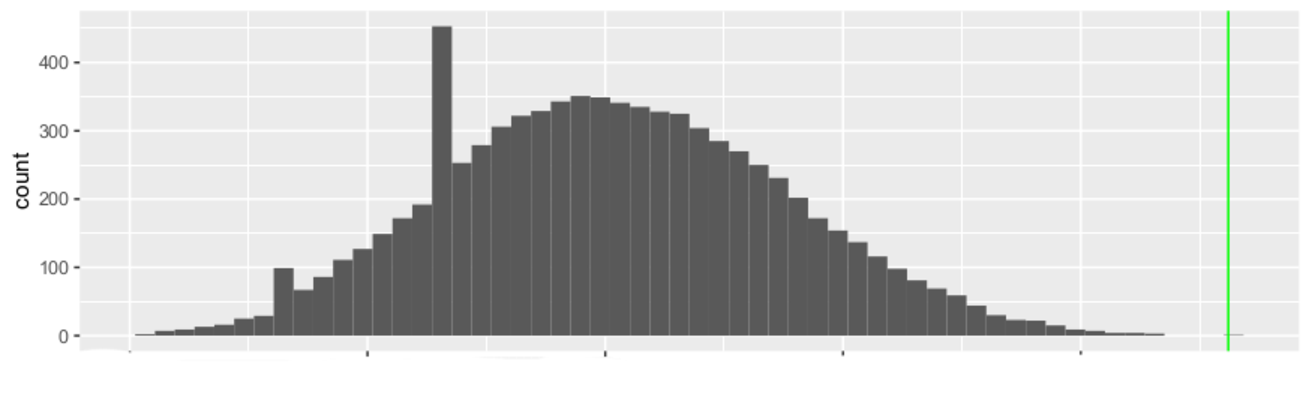
\includegraphics[width=5in]{height_ratios}
\end{figure}


\vspace{-0.2cm}\benum\truefalsesubquestionwithpoints{9} 

\begin{enumerate}[(a)]
\item The ratio of the sample averages is appropriate to test against the $H_0$ specified
\item The center of the null distribution should be close to 1
\item The center of the null distribution should be close to 0
\item The $B$ employed is too small to allow for valid inference
\item The $B$ employed is too large to allow for valid inference
\item For all reasonable $\alpha$, you can conclude the male height DGP is different from the female height DGP
\item Given the plot above (and if the $x$-axis grid was provided), you can approximate the retainment region for this test for $\alpha = 5\%$ by eye
\item The $p$ value is approximately 3\%
\item The 2-sample Kolmogorov-Smirnov test would likely have give us a different decision about $H_0$
\end{enumerate}
\eenum\instr\pagebreak

%%%%%%%%%%%%%%%%%%%%%%%%

\problem\timedsection{8} On midterm I you were given an example of a study that measured the lifespan of rats. Here is the raw data: 1.09, 2.48, 3.08, 2.57, 1.04, 0.87, 4.18, 2.23, 3.22, 1.33, 2.49, 1.69, 3.18, 1.39, 2.52, 4.8, 2.44, 1.47, 2.64, 3.96, 3.08, 2.71, 2.8, 3.4, 3.86, 2.28, 3.65, 3.28, 1.54, 1.94. We are now interested in not the mean lifespan but the 90\%ile lifespan. To investiage the 90\%ile lifespan, we employ the nonparametric bootstrap. Here is a frequency histogram of the values of the statistic calculated over $B = 1,000,000$ resamplings.

\begin{figure}[h]
\centering
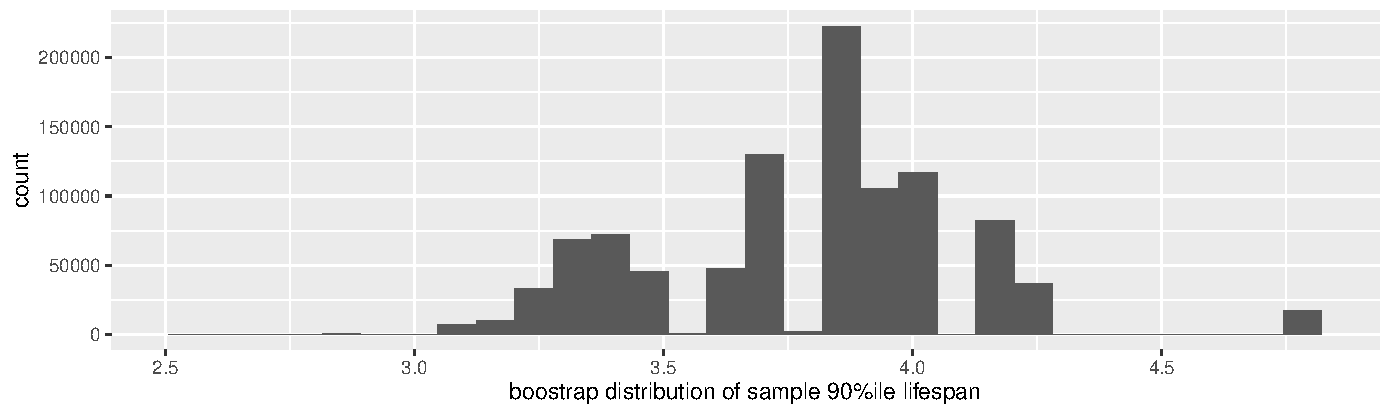
\includegraphics[width=5in]{bootstrap}
\end{figure}

\vspace{-0.2cm}\benum\truefalsesubquestionwithpoints{8} 

\begin{enumerate}[(a)]
\item The parameter of interest is the population 90\%ile lifespan
\item The statistic employed is the population 90\%ile lifespan
\item The boostrap is appropriate to study the 90\%ile lifespan
\item The boostrap resamplings constitute a \qu{null distribution}
\item The size of $B$ is appropriate for this scenario
\item An approximate 95\% CI for the population 90\%ile lifespan is between 2.5yr and 5yr
\item If you were testing against $H_0:$ the population 90\%ile lifespan is at most 3.5yr, this test would fail to reject $H_0$
\item If you were testing against $H_0:$ the population 90\%ile lifespan is at most 3.0yr, this test would fail to reject $H_0$
\end{enumerate}
\eenum\instr\pagebreak

%%%%%%%%%%%%%%%%%%%%%%%%

\problem\timedsection{11} On midterm I you were given an example of a study that measured the lifespan of rats in two scenarios: (scenario 1) low dose of magnesium and (scenario 2) high dose of magnesium. In (1) the low dose, $n_1=30$, $\xbar_1 = 2.57$ and $s_1 = 1.00$. In (2) the high dose, $n_2=6$, $\xbar_2 = 2.87$ and $s_2 = 1.11$. Let $\theta_2 - \theta_1$ be the difference between the mean high dose lifespan and the mean low dose lifespan. Rats were randomized into the two groups using the completely randomized design. Assume an additive treatment effect.

\vspace{-0.2cm}\benum\truefalsesubquestionwithpoints{14} 

\begin{enumerate}[(a)]
\item The study can be called an \qu{experiment}
\item This study has two arms
\item Each rat has two potential outcomes
\item The investigators are likely interested in a causal estimate for $\theta_2 - \theta_1$
\item A causal point estimate for $\theta_2 - \theta_1$ is $\xbar_2 - \xbar_1$
\item A 95\% CI for the treatment effect is $\approx \bracks{(\xbar_2 - \xbar_1) \pm 1.96 \times \se{\Xbar_2 - \Xbar_1}}$
\item Let $d$ be a correctly-calculated point estimate for $\theta_2 - \theta_1$; you can conclude that the high dose of magnesium causes an approximately $d$ difference in lifespan when compared to a low dose of magnesium
\item Causal estimation is not possible here due to the low sample size $n_2$
\item Causal estimation is not possible due to the high standard deviations
\item If the rats were not randomized, there could be confounders that could bias the causal point estimate
\item The mean point estimate over all randomizations will not have any bias due to confounders
\item In this particular assignment, there is no bias due to confounders
\item The number of assignments in this design is $\binom{30+6}{30}$
\item The difference in average noise between the two samples is near zero
\end{enumerate}
\eenum\instr\pagebreak

%%%%%%%%%%%%%%%%%%%%%%%%



\problem\timedsection{14} Consider $\Xoneton \iid \text{ShiftedParetoI}(1, \theta) := \theta (x + 1)^{-\theta - 1}$ which has support in positive real numbers only and a parameter space of $\theta > 0$. (You may remember this as the DPG from midterm II). Using calculus you can show that $\expe{X} = \frac{1}{\theta - 1}$. Let $u := \sum_{i=1}^n  \natlog{x_i + 1}$ and $U := \sum_{i=1}^n  \natlog{X_i + 1}$.

\vspace{-0.2cm}\benum\truefalsesubquestionwithpoints{17} 

\begin{enumerate}[(a)]
\item This DGP as stated has one parameter
\item $u > 0$
\item $u > n$
\item The likelihood is $u \theta^n$
\item The likelihood is $\theta^n \prod_{i=1}^n (x_i + 1)^{-\theta-1}$
\item The log-likelihood is $nu$
%\item The log-likelihood is $n\natlog{\theta} - (\theta + 1)u$
\item The log-likelihood is $n\natlog{\theta} - \theta u - u$
\item $\expe{X} \approx \thetahathatmle$
\item $\expe{X} \approx \xbar$
\item $\thetahathatmle = n / u$
\item $\thetahatmle = n / U$
\item The Fisher information is a function of $u$
\item The Fisher information cannot be computed for this DGP since its parameter space is $\neq \reals$
\item $I\parens{\thetahathatmle} = \tothepow{\thetahathatmle}{-2}$
\item $\thetahatmle$ is theoretically gauranteed to be unbiased based on properties of MLEs
\item $\ell(\thetahatmle, \xoneton)$ is theoretically gauranteed to be unbiased based on properties of MLEs
\item $\ell(\thetahathatmle, \xoneton)$ is the maximum value of the $\ell$ function
\end{enumerate}
\eenum\instr\pagebreak

%%%%%%%%%%%%%%%%%%%%%%%%

\problem\timedsection{9} \ingray{Consider $\Xoneton \iid \text{ShiftedParetoI}(1, \theta) := \theta (x + 1)^{-\theta - 1}$ which has support in positive real numbers only and a parameter space of $\theta > 0$. (You may remember this as the DPG from midterm II). Using calculus you can show that $\expe{X} = \frac{1}{\theta - 1}$. Let $u := \sum_{i=1}^n  \natlog{x_i + 1}$ and $U := \sum_{i=1}^n  \natlog{X_i + 1}$.} The following can be shown for this DGP:

\beqn
\ell(\theta, \xoneton) &=& n\natlog{\theta} - \theta u  -u, \\
\thetahathatmle &=& n / u, \\
I(\theta) &=& 1 / \theta^2
\eeqn

\noindent Consider the scenario where you are testing against $H_0: \theta = 1$ at $\alpha = 5\%$.% and with $n=58$ you calculate $u = 2.56$.

\vspace{-0.2cm}\benum\truefalsesubquestionwithpoints{9} 

\begin{enumerate}[(a)]
\item The log-likelihood under $H_0$ is $-2u$
\item The score function is $=n / \theta - u$
\item The Wald test rejects when $|n / u - 1| > 1.96$
\item The Score test rejects when $|n - u| > 1.96$
\item The Likelihood Ratio test rejects when $\sqrt{(n + u - n \natlog{n/u}) / u} > 1.96$
\item The Likelihood Ratio test rejects when $\sqrt{(n + u - n \natlog{n/u}) / (2u)} > 1.96$
\item The Likelihood Ratio test statistic is a draw from an approximate $\chisq{2}$ distribution
\item The Likelihood Ratio test statistic is a draw from an approximate $\chisq{n}$ distribution
\item The Likelihood Ratio test statistic is a draw from an approximate $\chisq{n - 1}$ distribution
%\item The Likelihood Ratio test rejects when $\sqrt{(n + u - n \natlog{n/u}) / u} > 1.96$
\end{enumerate}
\eenum\instr\pagebreak

%%%%%%%%%%%%%%%%%%%%%%%%

\problem\timedsection{14} \ingray{Consider $\Xoneton \iid \text{ShiftedParetoI}(1, \theta) := \theta (x + 1)^{-\theta - 1}$ which has support in positive real numbers only and a parameter space of $\theta > 0$. (You may remember this as the DPG from midterm II). Using calculus you can show that $\expe{X} = \frac{1}{\theta - 1}$. Let $u := \sum_{i=1}^n  \natlog{x_i + 1}$ and $U := \sum_{i=1}^n  \natlog{X_i + 1}$. The following can be shown for this DGP:

\beqn
\ell(\theta, \xoneton) &=& n\natlog{\theta} - \theta u  -u, \\
\thetahathatmle &=& n / u, \\
I(\theta) &=& 1 / \theta^2
\eeqn

\noindent Consider the scenario where you are testing against $H_0: \theta = 1$ at $\alpha = 5\%$.} You take a sample from the population of size $n=58$ and you calculate $u = 43.56$. All the following answers are accurate to three decimal places.


\vspace{-0.2cm}\benum\truefalsesubquestionwithpoints{13} 

\begin{enumerate}[(a)]
\item The Wald test statistic is 2.525
\item The Score test statistic is 2.525
\item The Likelihood Ratio test statistic is 2.525
\item The Wald test statistic is 2.166
\item The Score test statistic is 2.166
\item The Likelihood Ratio test statistic is 2.166
\item The Wald test statistic is 1.896
\item The Score test statistic is 1.896
\item The Likelihood Ratio test statistic is 1.896
\item The Wald, Score and Likelihood Ratio test statistics are equal in this DGP
\item The Wald, Score and Likelihood Ratio test statistics are equal in all DGPs
\item $CI_{\theta, 95\%} \approx \bracks{0.989, 1.674}$ to the nearest three decimals %true
\item $CI_{\theta, 95\%} \approx \bracks{1.074, 1.589}$ to the nearest three decimals
\end{enumerate}
\eenum\instr\pagebreak


\end{document}%%%%%%%%%%%%%%%%%%%%%%%
%%%%%%%%%%%%%%%%%%%%%%%%%%%%%%%
%%%%%%%%%%%%%%%%%%%%%%%%%%%%%%%
%%%%%%%%%%%%%%%%%%%%%%%%%%%%%%%
%%%%%%%%%%%%%%%%%%%%%%%%%%%%%%%
%%%%%%%%%%%%%%%%%%%%%%%%%%%%%%%
%%%%%%%%%%%%%%%%%%%%%%%%%%%%%%%
%%%%%%%%%%%%%%%%%%%%%%%%%%%%%%%
%%%%%%%%%%%%%%%%%%%%%%%%%%%%%%%
%%%%%%%%%%%%%%%%%%%%%%%%%%%%%%%
%%%%%%%%%%%%%%%%%%%%%%%%%%%%%%%
%%%%%%%%%%%%%%%%%%%%%%%%%%%%%%%
%%%%%%%%%%%%%%%%%%%%%%%%%%%%%%%
%%%%%%%%%%%%%%%%%%%%%%%%%%%%%%%
%%%%%%%%%%%%%%%%%%%%%%%%%%%%%%%
%%%%%%%%%%%%%%%%%%%%%%%%%%%%%%%
%%%%%%%%%%%%%%%%%%%%%%%%%%%%%%%
%%%%%%%%%%%%%%%%%%%%%%%%%%%%%%%
%%%%%%%%%%%%%%%%%%%%%%%%%%%%%%%
%%%%%%%%%%%%%%%%%%%%%%%%%%%%%%%
%%%%%%%%%%%%%%%%%%%%%%%%%%%%%%%
%%%%%%%%%%%%%%%%%%%%%%%%%%%%%%%

n = 58
u = 43.56
theta0 = 1
I_theta0 = 1

thetahathatmle = n/u
I_thetahathatmle = 1 / thetahathatmle^2

wald = (thetahathatmle - theta0) / sqrt(I_theta0^-1 / n)
round(wald, 3)
score = sqrt(n) - u / sqrt(n)
round(score, 3)
lik_rat = n * log(thetahathatmle) - n + u
round(lik_rat, 3)

badscore = (n - u) / (u / sqrt(n))
round(badscore, 3)

good_ci = c(
  thetahathatmle - 1.96 * sqrt(I_thetahathatmle^-1 / n),
  thetahathatmle + 1.96 * sqrt(I_thetahathatmle^-1 / n)
)
bad_ci = c(
  thetahathatmle - 1.96 * sqrt(I_theta0^-1 / n),
  thetahathatmle + 1.96 * sqrt(I_theta0^-1 / n)
)
round(good_ci,3)
round(bad_ci,3)


pacman::p_load(ggplot2)

diamonds

mod_red = lm(price ~ x + y + z + carat, diamonds)
mod_red

mod_full = lm(price ~ (x + y + z) * carat, diamonds)
mod_full

logLik(mod_full)
logLik(mod_red)
2 * (round(logLik(mod_full)) - round(logLik(mod_red)))

aic_red = -2 * round(logLik(mod_red)) + 2 * 6
aic_red
aic_full = -2 * round(logLik(mod_full)) + 2 * 6
aic_full

